\chapter{Construcción del sistema}
\label{cap:Construccion}

Este capítulo detalla la fase de construcción de la aplicación, comenzando con la toma de requistos, la toma de desiciones de diseño y culmina con la implementación.

\section{Toma de requisitos}
\label{sec:Requisitos}

Se han construido dos aplicaciones; La primera es el visualizador, el que se encarga de aplicar los filtros y mostrar la información correspondiente a los puntos donde se han detectado necesidades y la segunda corresponde a aquella que realiza la recepción del flujo de datos desde \textit{Twitter} y su paso por el clasificador. Las razones por las que se consideraron dos aplicaciones separadas se especificarán en la sección \ref{sec:Diseno}.\\

Esta sección detallará los requisitos de las aplicaciones, descritos como historias de usuario. Éstos señalan las necesidades de los clientes - Profesores guía y co-guía - expresadas en sucesivas reuniones mantenidas en el Departamento de Ingeniería Informática de la universidad donde se mostró, semana a semana, avances en la aplicación y se señalaron los cambios que habían de hacerse o que serían deseables.\\

Estos requisitos tendrán la siguiente nomenclatura para su identificación: Aquellos que guarden relación con la aplicación de detección se identificarán como 'HU-cXX' donde XX corresponderá al número del requisito; 'HU-vYY' para aquellas que correspondan a la aplicación interfáz donde, al igual que en el caso anterior, YY corresponderá al número del requisito.\\

La tabla ~\ref{tab:ReqTotales} presenta la totalidad de requisitos, tanto de la aplicación visualizador como del detector de necesitades.\\


\begin{table}[H]
\centering
\caption{Historias de usuario}
\label{tab:ReqTotales}
\begin{tabular}{cl}
\hline
\textbf{Identificador}       & \multicolumn{1}{c}{\textbf{Historia de usuario}}                                                                                                                                                                                                                                                                                                                                      \\ \hline
\multicolumn{1}{|c|}{HU-c00} & \multicolumn{1}{l|}{\begin{tabular}[c]{@{}l@{}}Como cliente quiero capturar necesidades de la población en tiempo real \\ cuando el país se encuentre en un escenario de catástrofe natural para poder \\ contar con información para asistir a la población afectada.\end{tabular}}                                                                                                  \\ \hline
\multicolumn{1}{|c|}{HU-c01} & \multicolumn{1}{l|}{\begin{tabular}[c]{@{}l@{}}Como cliente quiero que las necesidades detectadas se recojan desde la \\ información generadas en redes sociales redes sociales para que las personas\\ sean la fuente primaria.\end{tabular}}                                                                                                                                        \\ \hline
\multicolumn{1}{|c|}{HU-c02} & \multicolumn{1}{l|}{\begin{tabular}[c]{@{}l@{}}Como cliente quiero que la búsqueda de necesidades se vea enriquecida para\\  abarcar nuevos términos de búsqueda para abarcar un conjunto mayor de \\ información.\end{tabular}}                                                                                                                                                      \\ \hline
\multicolumn{1}{|c|}{HU-v00} & \multicolumn{1}{l|}{\begin{tabular}[c]{@{}l@{}}Como usuario quiero una interfaz donde pueda visualizar el comportamiento \\ del sistema de detección para poder interactuar con el.\end{tabular}}                                                                                                                                                                                     \\ \hline
\multicolumn{1}{|c|}{HU-v01} & \multicolumn{1}{l|}{\begin{tabular}[c]{@{}l@{}}Como cliente quiero que las necesidades detectadas puedan ser asociadas a \\ un punto en un mapa geográfico para poder identificar el lugar físico de su \\ fuente.\end{tabular}}                                                                                                                                                      \\ \hline
\multicolumn{1}{|c|}{HU-v02} & \multicolumn{1}{l|}{\begin{tabular}[c]{@{}l@{}}Como usuario quiero que puedan aplicarse filtros a la visualización de los \\ puntos de modo que según la distancia entre ellos, cuáles se quieran mostrar\\ y el nivel de acercamiento que tenga el mapa se entreguen diferentes formas\\ de mostrar la información para que la información se visualice con facilidad.\end{tabular}} \\ \hline
\multicolumn{1}{|c|}{HU-v03} & \multicolumn{1}{l|}{\begin{tabular}[c]{@{}l@{}}Como usuario quiero que la visualización de eventos se realice en tiempo \\ real para tomar decisiones rápidas cuando la situación lo amerite.\end{tabular}}                                                                                                                                                                           \\ \hline
\multicolumn{1}{|c|}{HU-v04} & \multicolumn{1}{l|}{\begin{tabular}[c]{@{}l@{}}Como usuario quiero visualizar eventos pasados, además quiero poder \\ seleccionar un intervalo de tiempo y que el sistema muestre todos los \\ eventos que se hayan detectado dentro de aquel intervalo de modo que \\ pueda realizarse una análisis a posteriori de la emergencia.\end{tabular}}                                     \\ \hline
\multicolumn{1}{|c|}{HU-v05} & \multicolumn{1}{l|}{\begin{tabular}[c]{@{}l@{}}Como usuario quiero poder especificar términos de búsqueda para acotar la\\  búsqueda a aquel contenido que contenga elementos que se correspondan \\ con ellos.\end{tabular}}                                                                                                                                                         \\ \hline
\multicolumn{1}{|c|}{HU-v06} & \multicolumn{1}{l|}{\begin{tabular}[c]{@{}l@{}}Como usuario quiero que cada punto, correspondiente a una necesidad \\ específica, tenga un diseño particular fácilmente identificable.\end{tabular}}                                                                                                                                                                                  \\ \hline
\multicolumn{1}{|c|}{HU-07}  & \multicolumn{1}{l|}{\begin{tabular}[c]{@{}l@{}}Como usuario quiero que sea posible visualizar estadísticas del procesamiento\\ de la aplicación por consulta.\end{tabular}}                                                                                                                                                                                                           \\ \hline
\multicolumn{1}{|c|}{HU-08}  & \multicolumn{1}{l|}{\begin{tabular}[c]{@{}l@{}}Como usuario quiero poder modificar cuánto tiempo se visualizará un evento \\ antes de que sea considerado antiguo y cada cuánto tiempo se añadirá la\\ información de los nuevos eventos.\end{tabular}}                                                                                                                               \\ \hline
\end{tabular}
\end{table}

Estas historias de usuario se corresponden con los criterios de aceptación descritos en la tabla ~\ref{tab:criteriosAceptacion} que se presenta a continuación.

\textbf{Faltan criterios, conversarlo con profes}

\section{Desiciones de diseño}
\label{sec:Diseno}

El desarrollo de la aplicación, entonces, será guiado por cumplir las historias de usuario descritas en la tabla ~\ref{tab:ReqTotales}. Para ello se trata cada historia como un problema individual que luego han de ser constituidas en la aplicación final. A continuación se presenta cómo se abordó cada historia desde el punto de vista del diseño para llevarla a su implementación descrita en el capítulo siguiente. Además se entrega una visión de la arquitectura final del sistema.\\

\subsection{Historia de usuario HU-c00}
\label{subsec:HU-c00}

Dado el contexto del funcionamiento del sistema, éste ha de entregar respuestas rápidas ante una emergencia; para ello, y como es descrito en esta historia de usuario, se requiere de un sistema capaz de procesar eventos en tiempo real que, dado el \textit{peak} de información que recibirá el sistema deberá ser escalable. El problema en este punto es el cómo construir un sistema que cumpla esta función y tenga esta, no menor, característica.\\

En primer lugar se consideraron sistemas de procesamiento distribuido; estos sistemas tienen la particularidad de ser una red de computadores (nodos, en general), que el usuario percibe como un solo gran sistema. Estos sistemas pueden ser de diversos tamaños, y suelen ser confiables, pues si un componente (nodo) falla, otro será capaz de reemplazarlo. \cite{DefSPD}. En un inicio se consideraron tres plataformas sobre las cuales podría construirse un sistema que pudiese cumplir con lo solicitado; dichas plataformas fueron Apache S4, Apache Storm y Apache Spark.\\

Apache S4, pese a su simplicidad, no continuó con su desarrollo luego del año 2013 y nunca tuvo una versión estable 1.0, razones por las cuales se dejó como segunda opción. Apache Spark, pese a contar con continuos \textit{releases}, una comunidad de desarrolladores no menor y permitir la elaboración de sistemas escalables no era lo que se buscaba en aquel momento como herramienta de desarrollo. Por ello finalmente se optó por Apache Storm; Storm permite construir sistemas que cumplan con las características de un sistema distribuido, como lo son: Escalabilidad (Tanto horizontal como vertical) y tolerancia a fallos (como la capacidad de un sistema para realizar correctamente y en todo momento aquello para lo que fue diseñado). Estos sistemas estan compuestos por dos tipos de elementos: Spout y Bolt, que fueron descritos en el Capítulo ~\ref{cap:MarcTeorico}. Al combinar esos elementos se da origen a un grafo dirigido, como el presentado en la Figura ~\ref{fig:stormBeLike} en la página ~\pageref{fig:stormBeLike}, donde cada elemento de procesamiento (\textit{bolt}), cumple con una determinada tarea utilizando como entrada la salida del elemento anterior.\\

Teniendo ya en consideración lo anterior el problema se traducía en cuál debería ser el procesamiendo que ha de aplicarse a los datos de entrada para capturar las necesidades. En primer lugar habrá que definir cuál y cómo será o serán las entradas del sistema para continuar la definición de los elementos con posterioridad.\\

\subsection{Historia de usuario HU-c01}
 \label{subsec:HU-c01}

La misma historia refleja desde dónde se obtendrán los datos, pero es necesario especificar más aún. Como se señaló al momento de definir los alcances de este trabajo, sólo se utilizará \textit{Twitter} como fuente de información, así la unidad de información pasará, desde ahora, a llamarse como se habitúa en aquella red social: \textit{Tweet}.\\

El asunto es, entonces, el cómo obtener la información que está produciéndose en \textit{Twitter} en tiempo real. Esta red social ha implementado una serie de interfaces para permitir a los desarrolladores acceder a sus datos; en particular, la \textit{Streaming API}, es aquella que permite acceder a la información de \textit{Twitter} con baja latencia. \cite{TwitterStreamingAPI}.\\

Existen tres tipos de \textit{streaming endpoints} disponibles, cada uno para un caso de uso particular:

\begin{table}[H]
\centering
\caption{\textit{Streaming endpoints} de \textit{Twitter}}
\label{StreamingEndpoints}
\begin{tabular}{|l|l|}
\hline
Público & \begin{tabular}[c]{@{}l@{}}Stream del que fluye la información pública de Twitter.\\ Casos de uso: Seguimiento de usuarios o tópicos específicos o minería de datos.\end{tabular} \\ \hline
Usuario & Flujo que toda la información correspondiente a un usuario.                                                                                                                       \\ \hline
Sitio   & Versión multi-usuario de la anterior.                                                                                                                                             \\ \hline
\end{tabular}
\end{table}

Para esta aplicación la adecuada corresponde a la API pública. Es ésta, a la vez, existen, básicamente, dos puntos de acceso: el público y \textit{firehose}. El acceso público es gratuito y permite el acceso a un 1\% de la información que se genera en tiempo real y para acceder a el basta con crear una aplicación dentro de \textit{Twitter}. En cambio para acceder a \textit{firehose}, el cual permite acceso total a la información, debe comprarse el acceso. Dadas estas condiciones se seleccionó, previo acuerdo con los clientes, el uso de la API pública.\\

Para hacer uso de la API descrita con anterioridad es necesario obtener cuatro claves de acceso: \textit{Access Token}, \textit{Access Token Secret}, \textit{Consumer Key (API Key)} y \textit{Consumer Secret (API Secret)}. Para más información sobre cómo conseguir estas claves consulte el Anexo ~\ref{anexo:TwitterKeys}.\\

Conociendo desde donde se obtendrá la información y teniendo acceso a ella resta conocer cómo realizar la conexión. Para ello se selecciono utilizar \textit{Twitter4J}, una biblioteca no oficial de Java para las API de \textit{Twitter}. Para su funcionamiento sólo requiere del uso de Java en su version 5 o superior.\\

El detalle de la implementación puede verse en la sección ~\ref{subsec:HU-c01Implementacion} en el Capítulo ~\ref{cap:Implementacion}.

\subsection{Historia de usuario HU-c02}
\label{subsec:HU-c02}

Esta historia de usuario guarda relación con la HU ~\ref{subsec:HU-v05}, menciona la necesidad de incrementar los términos de búsqueda para enriquecerla y abarcar la mayor información posible dado una consulta. Para realizar esto se consideró una práctica del procesamiento de lenguaje natural como es la denominada \textit{Query Expansion} (QE). Según lo descrito por \cite{IRQE} son técnicas comunes al utilizar QE la búsqueda de sinónimos (uso de diccionarios priviamente establecidos), diccionarios basados en la minería de los elementos previamente hayados, creación de diccionadios basados en la co-ocurrencia de términos, es decir, términos que suelen venir juntos o un vocabulario mantenido por editores humanos. Para este trabajo sólo se considerarán las dos primeras: Búsqueda por diccionario de sinónimos y una implementación que encuentra los términos más frecuentes dentro de los resultados de la búsqueda.\\

El diccionario de sinónimos es básicamente una bolsa de palabras asociadas a una semilla, es decir, dado un término de búsqueda agregar todos los términos asociados a el en el diccionario.\\

En el caso de la búsqueda de términos frecuentes....

\subsection{Historia de usuario HU-v00}
\label{subsec:HU-v00}

Dado que una topología de Apache Storm debe ser ejecutada de una forma particular y puede funcionar tanto en un cluster determinado como localmente el integrar la detección de necesidades con un \textit{framework} para construir la interfaz complica el desarrollo. Por ello se decidió separar la visualización y la detección en dos aplicaciones separadas que trabajasen juntas.\\

Teniendo en consideración la característica del desarrollo de esta aplicación como un proyecto ágil con un mínimo de personal para desarrollar se requería de un \textit{framework} que contribuyera a acelerar la construcción de la aplicación. Tras considerar las alternativas más conocidas como \textit{Spring}, \textit{Hibernate} o \textit{JSF} que tienen una curva de aprendizaje elevada, se optó por utilizar un cuarto \textit{framework} que aunque desconocido, prometía una simplicidad en su uso. \textit{Play Framework}, construido haciendo uso de Scala y Java permite construir aplicaciones ligeras (tamaño en disco), sin estado (no guarda configuraciones de una sesión para ser utilizadas luego) y por defecto RESTful, ideal para la comunicación entre aplicaciones. Éste \textit{framework} sigue el patrón de arquitectura Modelo-vista-controlador (MVC). Cuenta con un compilador en tiempo real (compila y realiza el despliegue de la aplicación cuando detecta un cambio en el código), lo que agiliza en gran medida el desarrollo, pues al automatizar este proceso mantiene la atención en lo que se está desarrollando.\\

Para visualizar los puntos encontrados por el detector de necesidades se decidió utilizar la API de \textit{Google Maps} la que permite la colocación de los denominados 'marcadores' en un punto específico del mapa y asociar a ellos algún tipo de información.\\

\subsection{Historia de usuario HU-v01}
\label{subsec:HU-v01}

Tal como se menciono con respecto a la historia de usuario anterior con el uso de \textit{Google Maps}, ésta historia se completará haciendo uso de los marcadores provistos por esta API.\\

\subsection{Historia de usuario HU-v02}
\label{subsec:HU-v02}

Desde el punto de vista ingenieríl no presenta mayor desafío, pero sí para fines prácticos. Se prepararon dos tipos de filtro: El primero considera el agrupamiento, mientras que el segundo considera el tipo de marcador.\\

Para el caso del agrupamiento se definieron tres modos de funcionamiento las cuales se describen a continuación:

\begin{enumerate}
\item No agrupar: Muestra todos los marcadores que correspondan en el mapa de acuerdo al punto geográfico que corresponda en su definición.
\item Agrupar por distancia: Define una grilla invisible en el mapa donde los elementos que calcen en una cudrícula son agregados a un \textit{cluster} y visualizados como tal.
\item Agrupar por categoría: Funciona de igual manera que el agrupamiento por distancia, pero sólo agrega elementos que comparan categoría.
\end{enumerate}

Para el segundo caso sólo se definieron dos reglas de funcionamiento las cuales se describen a continuación:

\begin{enumerate}
\item Mostrar todos: Muestra elementos de todas las categorias existentes.
\item Mostrar categoría: Para cada categoría mostrar sólo los elementos de aquella categoría. 
\end{enumerate}

Al combinar ambos tipos de filtros se tienen potencialmente seis modos de funcionamiento, pero considerando las categorías descritas en al sección ~\ref{subsec:categorias} ese número se expande a veintiún modos de funcionamiento del visualizador.\\

El detalle sobre la implementación puede verse en la sección ~\ref{subsec:HU-v02Implementacion} en el Capítulo ~\ref{cap:Implementacion}.\\

\subsection{Historia de usuario HU-v03}
\label{subsec:HU-v03}

Se solicitó que la interfaz no se recargue cada vez que se produzca un cambio dado por un nuevo evento detectado o el modificación en el intervalo de visualización. Para ello se utilizaron las facultados de Javascript y AJAX capturando los cambios en la línea temporal, descita en la HU-v04, y verificando la nueva información agregada.

\subsection{Historia de usuario HU-v04}
\label{subsec:HU-v04}

Al hacer referencia a información pasada se infiere la necesidad de la implementación de un sistema de persistencia de datos.\\

Para ello se consideraron los principales sistemas de bases de datos utilizados y conocidos por el autor, dentro de los cuales se encontraban herramientas como: MySQL, PostgreSQL, SQL Server, MongoDB, entre otras. Dadas las características y las condiciones con las cuales operará el sistema de detección se requiere de un DBMS con rápido tiempo de respuesta en operaciones lectura/escritura; la desición se tomó en base a los datos que se manejaran, pues no se apreció necesidad de implementar una base de datos relacional (véase sección \cite{subsec:BaseDeDatos}), de esta forma y teniendo en cuenta los resultados presentados en pruebas empíricas realizadas por \cite{MongoPerformance} en las cuales mostró que el tiempo de respuesta (en operaciones de lectura) es significativamente menor en MongoDB que en dos de los DBMS más conocidos como MySQL y PostgreSQL. Lo anterior, sumado al hecho de la capacidad de escalar de MongoDB reportada en fuentes oficiales o por diversos desarrolladores como \cite{MongoDBScalability} que han compartido sus experiencias en la \textit{web}, llevaron a decidir que mongo debiera ser el sistema de gestión de base de datos que se utilizase en el sistema.\\

Volviendo al punto; la necesidad de visualizar eventos pasados que involucró la participación de un sistema para persistir los datos, habiendo resuelto lo anterior la siguiente problemática se presenta como ¿qué datos han de guardarse? Según la definición de la historia en la que se señalan "eventos pasados dentro de un intervalo de tiempo", se infiera que ha de guardarse tanto el contenido visible del dato, la clasificación que se le asignó y la fecha en que se identificó, para ello y dado que se seleccionó MongoDB, y aunque no es necesario, se especificó un esquema para los documentos de la colección, pero ¿qué colección? dados los datos que se almacenarán sólo restaría tener la información correspondiente a la ubicación, por lo que el esquema se definió como se presenta en la Figura ~\nameref{fig:esquemaMarker1} correspondiente a la colección "Markers".

\begin{figure}[H]
	\centering
	\captionsetup{justification=centering}
	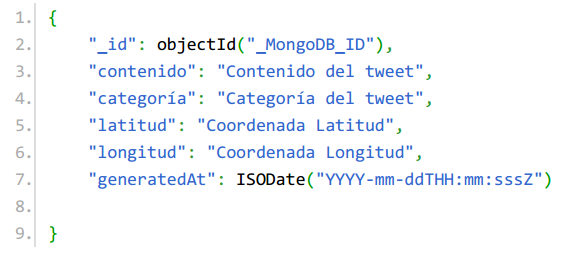
\includegraphics[scale=0.8]{images/Marker1.png}
	\caption[Ejemplo de documento en la colección Markers.]{Ejemplo de documento en la colección Markers.}
	\label{fig:esquemaMarker1}
\end{figure}

Parte de esta historia corresponde a la selección de un intervalo, los detalles de la implementación y la desición del diseño definitivo adoptado en la construcción se abordará la sección ~\ref{subsec:HU-v04Implementacion}.

\subsection{Historia de usuario HU-v05}
\label{subsec:HU-v05}

\textit{Twitter4J}, la herremienta que se mencionó en la sección ~\ref{subsec:HU-v01} como aquella que permitiría obtener el flujo de información desde \textit{Twitter} implementa una forma de filtrado mediante el uso de palabras clave, pero posee la limitante al momento de modificar la búsqueda, deben instanciarse nuevamente los objetos con los cuales se realiza la conexión a la API de \textit{Twitter}, eso se traduce en tiempo de procesamiento perdido, para solucionar este inconveniente se decidió implementar un operador, adicional a los apreciables en la sección ~\ref{subsec:definicionOperadores}, el cual estará encargado de realizar el filtrado de acuerdo a términos y llevar a cabo la operación descrita en la sección ~\ref{subsec:HU-c02} referente a la expansión de la consulta, pero siendo un operador significa que sea paralelizado y no exista una sola instancia ¿Cómo comunicar el estado de una consulta y que todos los operadores utilicen el mismo filtro?.\\

Nuevamente la respuesta consistió en recurrir a la base de datos; almacenar la consulta y asignar un estado para controlar el comportamiento del operador. Así el esquema en la base de datos queda tal y como se presenta en la Figura ~\nameref{fig:esquemaQuery}, documento de la colección "Queries".

\begin{figure}[H]
	\centering
	\captionsetup{justification=centering}
	\includegraphics[scale=0.8]{images/Query.png}
	\caption[Ejemplo de documento en la colección queries.]{Ejemplo de documento en la colección queries.}
	\label{fig:esquemaQuery}
\end{figure}

Donde la propiedad "estado" puede tomar dos valores: "actual" o "antiguo", reflejan si una consulta se está llevando a cabo o no. Estos valores son asignados por la aplicación responsable de la interfaz la responsable de recibir los términos de búsqueda por parte del usuario.

La implementación tanto de este operador como de las soluciones descritas en la sección ~\ref{subsec:HU-c02} pueden verse en la sección ~\ref{subsec:HU-c02Implementacion} y ~\ref{subsec:HU-v05Implementacion}.











